\documentclass[11pt,a4paper]{article}

% Packages
\usepackage[utf8]{inputenc}
\usepackage[T1]{fontenc}
\usepackage{geometry}
\geometry{margin=1in}
\usepackage{graphicx}
\usepackage{amsmath,amssymb}
\usepackage{booktabs}
\usepackage{hyperref}
\usepackage{xcolor}
\usepackage{listings}
\usepackage{caption}
\usepackage{subcaption}
\usepackage{float}
\usepackage{enumitem}
\usepackage{multirow}
\usepackage{array}
\usepackage{tikz}
\usetikzlibrary{shapes,arrows.meta,positioning,calc,fit,backgrounds}
\usepackage{pgfplots}
\pgfplotsset{compat=1.18}
\usepackage{algorithm}
\usepackage{algpseudocode}

% Code listing style
\lstset{
  language=Python,
  basicstyle=\ttfamily\small,
  keywordstyle=\color{blue}\bfseries,
  commentstyle=\color{gray}\itshape,
  stringstyle=\color{red!60!black},
  numbers=left,
  numberstyle=\tiny\color{gray},
  numbersep=5pt,
  frame=single,
  breaklines=true,
  captionpos=b,
  tabsize=2,
  showstringspaces=false,
}

\hypersetup{
  colorlinks=true,
  linkcolor=blue!60!black,
  citecolor=green!50!black,
  urlcolor=blue!70!black,
}

\title{
  \vspace{-1cm}
  \textbf{Bimanual Reaching for the Unitree G1 Humanoid:}\\[6pt]
  \large Reinforcement Learning with Joint-Space Control, \\
  Multi-Level Reward Shaping, and Sim-to-Real Transfer\\[12pt]
  \normalsize Technical Report
}
\author{
  Jonas\\
  Amber Robotics / Enactic, Inc.
}
\date{March 2026}

\begin{document}
\maketitle

\begin{abstract}
We present a complete reinforcement learning pipeline for bimanual 6-DOF pose reaching on the Unitree G1 humanoid robot. Starting from an initial IK-based approach, we iteratively developed a direct joint-space control policy using Proximal Policy Optimization (PPO) trained in Isaac Lab 5.1.0 with 4,096 parallel environments. Over approximately 17 training runs spanning multiple weeks, we systematically discovered and resolved critical issues including unreachable workspace targets, cross-arm reward interference, action-based reward incompatibility with orientation control, shared-network gradient imbalance in bimanual learning, and position-orientation reward trade-offs. The final policy achieves \textbf{1.7--5.8\,cm position error} and \textbf{0.028--0.039\,rad ($\sim$1.6--2.2$^\circ$) orientation error} for both arms simultaneously, with randomized 6-DOF pose targets within the robot's reachable workspace. Key contributions include a novel \emph{bimanual balance reward} using per-element minimum aggregation across arms, multi-level orientation tracking rewards with appropriately scaled tanh kernels, and the identification that action-magnitude penalties are fundamentally incompatible with orientation control in shared-network bimanual architectures. The trained policy is deployed on real hardware via direct joint-space commands at 50\,Hz with an integrated emergency-stop system.
\end{abstract}

\tableofcontents
\newpage

%% ============================================================
\section{Introduction and Motivation}
\label{sec:intro}

Humanoid robots are increasingly deployed in unstructured environments requiring dexterous bimanual manipulation. The Unitree G1 is a full-size humanoid with a 29-DOF body, of which we control the 14 upper-body degrees of freedom (7 per arm: shoulder pitch/roll/yaw, elbow, wrist roll/pitch/yaw). The fundamental task---reaching arbitrary 6-DOF poses with both hands simultaneously---is a prerequisite for grasping, handover, and contact-rich manipulation.

\subsection{Why Reinforcement Learning?}
Classical approaches to bimanual reaching rely on inverse kinematics (IK) solvers, which are effective for position-only targets but struggle with:
\begin{itemize}[nosep]
  \item Joint-limit awareness and singularity avoidance,
  \item Simultaneous position \emph{and} orientation control with 7-DOF redundancy,
  \item Smooth, jitter-free trajectories suitable for real hardware,
  \item Sim-to-real transfer without hand-tuned controllers.
\end{itemize}
Reinforcement learning (RL) addresses these by learning a single neural network policy that maps observations to joint-space actions, directly deployable on hardware without any kinematic solver at runtime.

\subsection{Project Scope}
This report covers the full development arc:
\begin{enumerate}[nosep]
  \item Initial IK-based control baseline (position-only, 6D action space),
  \item Transition to direct joint-space control (14D action space),
  \item Reward engineering for position tracking with anti-jitter properties,
  \item Extension to full 6-DOF pose (position + orientation) with randomized targets,
  \item Discovery and resolution of bimanual gradient imbalance,
  \item Deployment on real G1 hardware with safety systems.
\end{enumerate}

%% ============================================================
\section{Background and Related Work}
\label{sec:background}

\subsection{Proximal Policy Optimization (PPO)}
PPO~\cite{schulman2017ppo} is an on-policy actor-critic algorithm that optimizes a clipped surrogate objective:
\begin{equation}
  L^{\text{CLIP}}(\theta) = \hat{\mathbb{E}}_t\left[\min\left(r_t(\theta)\hat{A}_t,\;\text{clip}(r_t(\theta), 1-\epsilon, 1+\epsilon)\hat{A}_t\right)\right]
\end{equation}
where $r_t(\theta) = \frac{\pi_\theta(a_t|s_t)}{\pi_{\theta_{\text{old}}}(a_t|s_t)}$ is the probability ratio and $\hat{A}_t$ is the estimated advantage. We use the RSL-RL implementation with $\epsilon=0.2$, Generalized Advantage Estimation (GAE, $\lambda=0.97$, $\gamma=0.99$), and an adaptive learning rate schedule targeting $\text{KL}=0.01$.

\subsection{Isaac Lab and Massively Parallel Simulation}
Isaac Lab 5.1.0~\cite{isaaclab} provides GPU-accelerated physics simulation via NVIDIA Isaac Sim. We train with 4,096 parallel environments on a single RTX 4090 GPU, achieving approximately 1.3 million environment steps per second. The \texttt{ManagerBasedRLEnv} architecture allows modular specification of observations, rewards, actions, events, and terminations through Python configuration classes.

\subsection{Sim-to-Real Transfer}
Direct joint-space control (as opposed to task-space/IK-based control) simplifies sim-to-real transfer because the policy's output---joint position deltas---can be applied directly to the robot's PD controllers without runtime kinematic computations. Domain randomization on joint reset positions ($\pm$0.15\,rad) and base pose ($\pm$0.02\,m, $\pm$0.05\,rad yaw) further improves robustness.

%% ============================================================
\section{System Architecture}
\label{sec:architecture}

\subsection{Robot Configuration}
The G1 upper body is configured as a 14-DOF articulation with a fixed base (\texttt{waist\_yaw\_link}). Table~\ref{tab:joint_config} summarizes the joint properties.

\begin{table}[H]
\centering
\caption{G1 Upper Body Joint Configuration (per arm)}
\label{tab:joint_config}
\begin{tabular}{@{}llcccc@{}}
\toprule
\textbf{Joint Group} & \textbf{Joints} & \textbf{$K_p$} & \textbf{$K_d$} & \textbf{Effort (Nm)} & \textbf{Vel (rad/s)} \\
\midrule
Shoulders & pitch, roll, yaw & 300 & 100 & 25.0 & 20.0 \\
Elbow & pitch & 300 & 100 & 25.0 & 20.0 \\
Wrists & roll, pitch, yaw & 200 & 80 & 5.0 & 15.0 \\
\bottomrule
\end{tabular}
\end{table}

\noindent End-effector frames are defined at \texttt{left\_rubber\_hand} and \texttt{right\_rubber\_hand}. The simulation runs at 100\,Hz ($dt=0.01$\,s) with control decimation of 2, yielding an effective 50\,Hz policy frequency.

\subsection{Policy Network Architecture}

% Architecture diagram
\begin{figure}[H]
\centering
\begin{tikzpicture}[
  layer/.style={draw, rounded corners, minimum width=3.5cm, minimum height=0.7cm, fill=blue!10, font=\small},
  obs/.style={draw, rounded corners, minimum width=2.4cm, minimum height=0.55cm, fill=green!10, font=\scriptsize},
  out/.style={draw, rounded corners, minimum width=3.5cm, minimum height=0.7cm, fill=red!10, font=\small},
  arrow/.style={-Stealth, thick},
]

% Observations (left column)
\node[obs] (jpos) at (-4.2, 4.0) {Joint Pos Rel (14D)};
\node[obs] (jvel) at (-4.2, 3.2) {Joint Vel (14D)};
\node[obs] (lpe)  at (-4.2, 2.4) {Left EE Pos Err (3D)};
\node[obs] (rpe)  at (-4.2, 1.6) {Right EE Pos Err (3D)};
\node[obs] (loe)  at (-4.2, 0.8) {Left EE Orient Err (3D)};
\node[obs] (roe)  at (-4.2, 0.0) {Right EE Orient Err (3D)};
\node[obs] (lev)  at (-4.2, -0.8) {Left EE Vel (3D)};
\node[obs] (rev)  at (-4.2, -1.6) {Right EE Vel (3D)};
\node[obs] (act)  at (-4.2, -2.4) {Last Action (14D)};

% Obs normalization
\node[layer, fill=yellow!15, minimum width=2.4cm] (norm) at (-0.5, 1.0) {\footnotesize Running Norm};

% MLP Layers
\node[layer] (h1) at (2.5, 3.0) {FC 512 + ELU};
\node[layer] (h2) at (2.5, 1.5) {FC 256 + ELU};
\node[layer] (h3) at (2.5, 0.0) {FC 256 + ELU};

% Outputs
\node[out] (act_out) at (2.5, -1.8) {Actions (14D)};
\node[font=\scriptsize, text=gray] at (2.5, -2.4) {$\times$ 0.03 rad scale};

% Arrows from obs to norm
\foreach \n in {jpos, jvel, lpe, rpe, loe, roe, lev, rev, act} {
  \draw[arrow, gray!60] (\n.east) -- (norm.west|-\n.east);
}

% Arrows through MLP
\draw[arrow] (norm.east) -- ++(0.5,0) |- (h1.west);
\draw[arrow] (h1) -- (h2);
\draw[arrow] (h2) -- (h3);
\draw[arrow] (h3) -- (act_out);

% Label
\node[font=\bfseries\small, anchor=south] at (-4.2, 4.6) {Observations (60D)};
\node[font=\bfseries\small, anchor=south] at (2.5, 3.6) {Actor MLP};

% Brace for obs
\draw[decorate, decoration={brace, amplitude=4pt, mirror}] (-5.8, -2.7) -- (-5.8, 4.3) node[midway, left=6pt, font=\scriptsize, rotate=90] {60 dims};
\end{tikzpicture}
\caption{Actor network architecture. The critic shares the same topology but outputs a scalar value estimate. Observations are normalized via running mean/std statistics accumulated during training.}
\label{fig:network_arch}
\end{figure}

\noindent The policy uses an MLP with hidden dimensions $[512, 256, 256]$ and ELU activations. Both actor and critic use empirical observation normalization. The actor outputs 14D joint position deltas scaled by 0.03\,rad, applied relative to default joint positions via a PD controller. The network has approximately 330K trainable parameters.

\subsection{Observation Space}
The observation vector (60D) is designed for clear arm-target association:
\begin{equation}
  \mathbf{o} = [\underbrace{\Delta\mathbf{q}}_{\text{14D joint pos}},\;\underbrace{\dot{\mathbf{q}}}_{\text{14D joint vel}},\;\underbrace{\mathbf{e}_L^{\text{pos}}}_{\text{3D}},\;\underbrace{\mathbf{e}_R^{\text{pos}}}_{\text{3D}},\;\underbrace{\mathbf{e}_L^{\text{orient}}}_{\text{3D}},\;\underbrace{\mathbf{e}_R^{\text{orient}}}_{\text{3D}},\;\underbrace{\dot{\mathbf{x}}_L}_{\text{3D}},\;\underbrace{\dot{\mathbf{x}}_R}_{\text{3D}},\;\underbrace{\mathbf{a}_{t-1}}_{\text{14D last action}}]
\end{equation}
where $\mathbf{e}^{\text{pos}} = \mathbf{x}^{\text{des}} - \mathbf{x}^{\text{curr}}$ is the position error and $\mathbf{e}^{\text{orient}} = \text{quat\_box\_minus}(\mathbf{q}^{\text{des}}, \mathbf{q}^{\text{curr}})$ is the 3D axis-angle orientation error.

%% ============================================================
\section{Workspace Analysis}
\label{sec:workspace}

A critical early discovery was that the initial target workspace contained unreachable poses.

\subsection{Arm Kinematics}
The G1's shoulder joint is located at approximately $(0.004, \pm0.100, 0.238)$\,m in the body frame. Through analysis of the URDF link lengths, we computed a maximum arm reach of approximately 0.41\,m from the shoulder joint.

\subsection{Original vs.\ Tightened Workspace}
\begin{table}[H]
\centering
\caption{Workspace bounds evolution (body frame, meters)}
\label{tab:workspace}
\begin{tabular}{@{}lcccc@{}}
\toprule
& \textbf{$x$ (forward)} & \textbf{$y$ (lateral)} & \textbf{$z$ (vertical)} & \textbf{Max dist.\ from shoulder} \\
\midrule
Original & $[0.20, 0.45]$ & $[\pm0.10, \pm0.30]$ & $[-0.15, 0.15]$ & 0.55\,m \\
Tightened & $[0.15, 0.30]$ & $[\pm0.05, \pm0.22]$ & $[0.05, 0.25]$ & 0.36\,m \\
\bottomrule
\end{tabular}
\end{table}

\noindent The original workspace corners were 0.55\,m from the shoulder---well beyond the 0.41\,m reach limit. After tightening, all target positions are within 0.36\,m, ensuring physical reachability. This single change reduced position error from $\sim$6\,cm to $\sim$1.8\,cm.

\begin{figure}[H]
\centering
% Placeholder for workspace diagram
\fbox{\parbox{0.85\textwidth}{\centering\vspace{3cm}\textit{[FIGURE: Workspace bounds visualization showing original (red) vs.\ tightened (green) target regions relative to arm reach sphere]}\vspace{3cm}}}
\caption{Workspace bounds relative to arm reachability. Red: original bounds with corners at 0.55\,m. Green: tightened bounds fully within 0.36\,m reach.}
\label{fig:workspace}
\end{figure}

%% ============================================================
\section{Reward Function Design}
\label{sec:rewards}

Reward engineering was the central challenge of this project. We detail the evolution through multiple design iterations.

\subsection{Multi-Level Position Tracking}
Position tracking uses three tanh-kernel rewards at different spatial scales:
\begin{equation}
  r_{\text{pos}}^{(k)} = w_k \cdot \left(1 - \tanh\left(\frac{\|\mathbf{x}^{\text{des}} - \mathbf{x}^{\text{curr}}\|}{\sigma_k}\right)\right)
  \label{eq:pos_tracking}
\end{equation}

\begin{table}[H]
\centering
\caption{Multi-level position tracking rewards (per arm)}
\label{tab:pos_rewards}
\begin{tabular}{@{}lccc@{}}
\toprule
\textbf{Level} & \textbf{$\sigma$ (m)} & \textbf{Weight $w$} & \textbf{Active Range} \\
\midrule
Coarse & 0.50 & 5.0 & All distances (gradient at 30+\,cm) \\
Medium & 0.25 & 6.0 & $<$15\,cm (gradient sharpens) \\
Fine   & 0.10 & 8.0 & $<$5\,cm (strong near-target pull) \\
\bottomrule
\end{tabular}
\end{table}

\noindent Additionally, a \emph{holding reward} ($w=5.0$, threshold 4\,cm) rewards low EE velocity when near target, and a \emph{success bonus} ($w=8.0$, threshold 3\,cm) provides a sparse binary reward.

\subsection{Multi-Level Orientation Tracking}
Orientation tracking mirrors the multi-level position approach:
\begin{equation}
  r_{\text{orient}}^{(k)} = w_k \cdot \left(1 - \tanh\left(\frac{\|\mathbf{e}^{\text{orient}}\|}{\sigma_k}\right)\right)
\end{equation}
where $\|\mathbf{e}^{\text{orient}}\| = \text{quat\_error\_magnitude}(\mathbf{q}^{\text{curr}}, \mathbf{q}^{\text{des}})$.

\begin{table}[H]
\centering
\caption{Multi-level orientation tracking rewards (per arm)}
\label{tab:orient_rewards}
\begin{tabular}{@{}lccc@{}}
\toprule
\textbf{Level} & \textbf{$\sigma$ (rad)} & \textbf{Weight $w$} & \textbf{Active Range} \\
\midrule
Coarse & 1.50 & 12.0 & All errors (gradient at 1--2\,rad) \\
Fine   & 0.30 & 15.0 & $<$0.5\,rad (strong sub-radian precision) \\
\bottomrule
\end{tabular}
\end{table}

\noindent The coarse orientation reward uses $\sigma=1.5$\,rad to ensure the tanh kernel does not saturate at large errors (a critical lesson---see Section~\ref{sec:orient_std}).

\subsection{Bimanual Balance Reward}
\label{sec:bimanual_balance}
The most important reward innovation was the \emph{bimanual balance reward}, which returns the minimum of both arms' tracking performance:
\begin{equation}
  r_{\text{bimanual}} = w \cdot \min\!\left(f(\mathbf{e}_L),\; f(\mathbf{e}_R)\right)
\end{equation}
where $f(\mathbf{e}) = 1 - \tanh(\|\mathbf{e}\|/\sigma)$. This reward can \emph{only} be increased by improving the worse-performing arm, eliminating the gradient imbalance that causes one arm to converge while the other stalls (Section~\ref{sec:gradient_imbalance}).

\begin{table}[H]
\centering
\caption{Bimanual balance rewards}
\label{tab:bimanual}
\begin{tabular}{@{}lccc@{}}
\toprule
\textbf{Term} & \textbf{Modality} & \textbf{$\sigma$} & \textbf{Weight} \\
\midrule
\texttt{bimanual\_pos\_coarse} & Position & 0.50\,m & 15.0 \\
\texttt{bimanual\_pos\_fine}   & Position & 0.10\,m & 20.0 \\
\texttt{bimanual\_orient}      & Orientation & 1.50\,rad & 25.0 \\
\bottomrule
\end{tabular}
\end{table}

\subsection{Regularization and Anti-Jitter Rewards}

\begin{table}[H]
\centering
\caption{Regularization and state-dependent reward terms}
\label{tab:regularization}
\begin{tabular}{@{}llc@{}}
\toprule
\textbf{Term} & \textbf{Description} & \textbf{Weight} \\
\midrule
\texttt{action\_rate\_l2} & Global action change penalty & $-0.2$ \\
\texttt{joint\_vel\_l2} & Joint velocity penalty & $-0.005$ \\
\texttt{joint\_acc\_l2} & Joint acceleration penalty & $-0.005$ \\
\texttt{flat\_orientation} & Base orientation penalty (roll, pitch) & $-1.0$ \\
\texttt{ee\_vel\_near\_target} & EE velocity near target (per arm) & $-8.0$ \\
\texttt{adaptive\_action\_rate} & Proximity-scaled action jitter (per arm) & $-0.2$ \\
\texttt{terminal\_damping} & Reward for stillness at target (per arm) & $+10.0$ \\
\bottomrule
\end{tabular}
\end{table}

\noindent The adaptive action rate penalty uses Gaussian proximity scaling:
\begin{equation}
  r_{\text{adapt}} = -w \cdot \exp\!\left(-\frac{d^2}{\sigma^2}\right) \cdot \sum_{i=i_{\text{start}}}^{i_{\text{end}}} (a_i^t - a_i^{t-1})^2
\end{equation}
where $d$ is the EE-to-target distance and $[i_{\text{start}}, i_{\text{end}})$ isolates the current arm's action dimensions (Section~\ref{sec:cross_arm}).

%% ============================================================
\section{Training Progression and Iterative Problem-Solving}
\label{sec:training}

This section chronicles the full sequence of training experiments, detailing each problem discovered and the corresponding fix.

\subsection{Phase 0: IK-Based Baseline}
The initial approach used a 6D action space (3D position delta per arm) with differential IK converting to joint commands at runtime. This achieved functional reaching but had inherent limitations:
\begin{itemize}[nosep]
  \item IK dependency prevents clean sim-to-real transfer,
  \item Position-only control (no orientation),
  \item Limited to 4-DOF per arm (shoulder + elbow; wrists fixed).
\end{itemize}
Result: functional but position-only, with IK dependency on hardware.

\subsection{Phase 1: Joint-Space Control (Position Only)}
\label{sec:phase1}
We switched to direct 14D joint-space control with the original reward configuration (action\_rate=$-0.5$, position tracking only). This eliminated IK dependency.

\begin{table}[H]
\centering
\caption{Phase 1 results: Joint-space control baseline}
\begin{tabular}{@{}lcc@{}}
\toprule
\textbf{Metric} & \textbf{Left Arm} & \textbf{Right Arm} \\
\midrule
Position error & $\sim$6.0\,cm & $\sim$6.4\,cm \\
Mean reward & \multicolumn{2}{c}{261.6} \\
Iterations & \multicolumn{2}{c}{5,000} \\
\bottomrule
\end{tabular}
\end{table}

\subsection{Phase 2 Curriculum: Anti-Jitter Rewards}
\label{sec:phase2}
To reduce wobble, we attempted a two-phase curriculum:
\begin{itemize}[nosep]
  \item \textbf{Phase 1}: Train with position tracking only for 5,000 iterations.
  \item \textbf{Phase 2}: Activate state-dependent anti-jitter rewards and resume training.
\end{itemize}

\paragraph{Attempt 1: Catastrophic Weights.}
Initial Phase 2 weights (\texttt{adaptive\_action\_rate}$=-4.0$, \texttt{proximity\_action\_mag}$=-3.0$) produced catastrophic episode costs of $-1,350$ to $-1,435$ per episode from \texttt{proximity\_action\_mag} alone, overwhelming all tracking rewards. Total mean reward collapsed to $-22,000$.

\paragraph{Attempt 2: Calibrated Weights.}
After computing raw reward magnitudes from logged data, we recalibrated (\texttt{adaptive\_action\_rate}$=-0.5$, \texttt{proximity\_action\_mag}$=-0.01$, \texttt{adaptive\_orientation}$=-5.0$). Position error regressed from 6\,cm to 9\,cm, but orientation improved ($0.89\to0.47$\,rad). The two-phase transition itself caused instability.

\textbf{Lesson:} Two-phase curricula are fragile. Activating new reward terms mid-training disrupts the learned value function.

\subsection{Single-Phase Training with Tightened Workspace}
\label{sec:single_phase}
We abandoned the curriculum approach and adopted single-phase training with all rewards active from the start. Combined with the workspace tightening (Section~\ref{sec:workspace}) and reduced action scale ($0.05\to0.03$\,rad):

\begin{table}[H]
\centering
\caption{Single-phase results (position only, tightened workspace)}
\begin{tabular}{@{}lcc@{}}
\toprule
\textbf{Metric} & \textbf{Left Arm} & \textbf{Right Arm} \\
\midrule
Position error & 1.8\,cm & 15.8\,cm \\
Mean reward & \multicolumn{2}{c}{$\sim$180} \\
\bottomrule
\end{tabular}
\end{table}

\noindent A severe left--right asymmetry emerged. Investigation revealed the \textbf{cross-arm interference bug} (Section~\ref{sec:cross_arm}).

\subsection{Cross-Arm Interference Bug}
\label{sec:cross_arm}
State-dependent rewards that used \texttt{env.action\_manager.action} (the full 14D vector) penalized \emph{all} joints when \emph{either} arm was near its target. When the left arm converged to 1.8\,cm, the Gaussian proximity factor $\approx 1.0$ for the left arm caused the penalty to suppress right arm actions [7:14] as well.

\paragraph{Fix:} Added \texttt{action\_start} and \texttt{action\_end} parameters to all action-based reward functions, slicing per-arm actions: left $[0:7]$, right $[7:14]$.

\begin{lstlisting}[caption={Per-arm action isolation in reward functions},label={lst:per_arm}]
def adaptive_action_rate_penalty(env, sigma, command_name,
    asset_cfg, action_start=0, action_end=7):
    distance = _compute_ee_distance(env, command_name, asset_cfg)
    proximity = torch.exp(-torch.square(distance / sigma))
    # Only THIS arm's actions
    action = env.action_manager.action[:, action_start:action_end]
    prev_action = env.action_manager.prev_action[:, action_start:action_end]
    action_rate_sq = torch.sum(torch.square(action - prev_action), dim=1)
    return proximity * action_rate_sq
\end{lstlisting}

\noindent After this fix, both arms converged to excellent position accuracy:

\begin{table}[H]
\centering
\caption{Results after cross-arm fix (position only)}
\begin{tabular}{@{}lcc@{}}
\toprule
\textbf{Metric} & \textbf{Left Arm} & \textbf{Right Arm} \\
\midrule
Position error & \textbf{1.5\,cm} & \textbf{1.8\,cm} \\
Orientation error & 1.22\,rad & 0.35\,rad \\
\bottomrule
\end{tabular}
\end{table}

\noindent Position was solved, but orientation remained poor---especially for the left arm (1.22\,rad $\approx 70^\circ$ constant offset).

\subsection{Adding Orientation Control}
\label{sec:orientation}

\subsubsection{Root Cause: No Orientation Observations}
The policy had no information about target orientation. The 54D observation space contained only position errors, joint states, and velocities---no orientation signal. The left arm's constant orientation offset resulted from the policy finding a joint configuration that minimized position error without any consideration for wrist alignment.

\subsubsection{Orientation Observation}
We added a 3D axis-angle orientation error observation per arm using the quaternion box-minus operator:

\begin{lstlisting}[caption={Orientation error observation},label={lst:orient_obs}]
def ee_orientation_error(env, command_name, asset_cfg):
    asset = env.scene[asset_cfg.name]
    command = env.command_manager.get_command(command_name)
    des_quat_b = command[:, 3:7]
    des_quat_w = quat_mul(asset.data.root_quat_w, des_quat_b)
    curr_quat_w = asset.data.body_quat_w[:, asset_cfg.body_ids[0]]
    return quat_box_minus(des_quat_w, curr_quat_w)  # 3D axis-angle
\end{lstlisting}

\noindent This increased the observation space from 54D to 60D.

\subsubsection{Target Orientation Randomization}
We randomized target orientations within physically achievable ranges:
\begin{equation}
  \text{roll} \in [-0.5, 0.5]\;\text{rad},\quad
  \text{pitch} \in [-0.3, 0.3]\;\text{rad},\quad
  \text{yaw} \in [-0.5, 0.5]\;\text{rad}
\end{equation}

\subsubsection{Orientation Penalty: Perverse Incentive}
The initial \texttt{adaptive\_orientation\_penalty} with weight $-5.0$ created a \emph{perverse incentive}: the proximity-scaled penalty meant the right arm avoided approaching its target to dodge the orientation penalty. Result: left arm 1.7\,cm position but right arm stuck at 17.5\,cm.

Reducing the weight to $-1.0$ did not fully resolve the issue---the right arm remained stuck at $\sim$23\,cm at iteration 5,520/10,000.

\subsection{Wrist Penalty Conflict}
\label{sec:wrist_conflict}
Analysis of the reward breakdown revealed \texttt{wrist\_position\_penalty} ($w=-0.8$, episode cost $-0.72$) was directly fighting orientation control. This penalty pushed wrist joints toward zero, but with randomized orientation targets, the wrists \emph{must} deviate from zero to achieve commanded orientations.

\textbf{Fix:} Removed both \texttt{wrist\_position\_penalty} and \texttt{wrist\_velocity\_penalty}.

\subsection{Global Action Rate Penalty}
\label{sec:action_rate}
The global \texttt{action\_rate\_l2} at weight $-1.0$ produced an episode cost of $-3.09$---the single largest penalty. Since this operates on all 14 joints, when one arm converges and holds still, the other arm's exploratory movements are penalized. At weight $-1.0$, the right arm's tracking reward ($\sim$3.36) barely exceeded its share of the action rate cost.

\textbf{Fix:} Reduced \texttt{action\_rate\_l2} weight from $-1.0$ to $-0.2$. The per-arm \texttt{adaptive\_action\_rate\_penalty} handles near-target jitter.

\subsection{Proximity Action Magnitude: Incompatible with Orientation}
\label{sec:prox_action}
After the above fixes, the right arm converged to 0.92\,cm---but the left arm stalled at 28\,cm. The reward breakdown showed \texttt{right\_proximity\_action\_mag} = $-7.38$ per episode (the largest penalty). At 1\,cm distance, the proximity factor $\approx 0.97$, penalizing \emph{all} action magnitude including wrist joint actions needed for orientation control.

Through the shared network's gradient flow, this ``be still'' gradient suppressed the left arm's ability to make the large movements needed to reach its target.

\textbf{Fix:} Removed \texttt{proximity\_action\_magnitude\_penalty} entirely. Also removed action magnitude from \texttt{terminal\_damping\_reward} (which multiplied by $\exp(-\|\mathbf{a}\| \cdot 5)$), since wrist actions are needed at target for orientation control.

\subsection{Shared-Network Gradient Imbalance}
\label{sec:gradient_imbalance}
Even after removing all action-based penalties, training continued to exhibit one-arm-converges-other-stalls behavior. Across 4 different training runs:

\begin{table}[H]
\centering
\caption{One-arm convergence pattern across training runs}
\begin{tabular}{@{}ccc@{}}
\toprule
\textbf{Run} & \textbf{Converged Arm} & \textbf{Stuck Arm Position} \\
\midrule
1 (per-arm action rate) & Right ($\sim$7\,cm) & Left (23\,cm) \\
2 (reduced action rate) & Right (2.5\,cm) & Left (24.7\,cm) \\
3 (removed prox. penalty) & Left (0.9\,cm) & Right (24.1\,cm) \\
4 (larger network) & Left (0.9\,cm) & Right (24.1\,cm) \\
\bottomrule
\end{tabular}
\end{table}

\noindent The pattern was consistent: whichever arm converged first accumulated high tracking rewards (38+ per episode), dominating the gradient over the lagging arm's weak signal (2--3 per episode). The shared network parameters were pulled by the dominant arm, effectively locking out the other.

This is a fundamental challenge of bimanual RL with shared networks: the actor produces \emph{both} arms' actions simultaneously, so gradients from one arm's rewards affect the other arm's output through shared weights.

\textbf{Fix:} The \emph{bimanual balance reward} (Section~\ref{sec:bimanual_balance}), which returns $\min(\text{left}, \text{right})$, eliminates this imbalance. When one arm is at 1\,cm and the other at 24\,cm, improving the converged arm yields zero marginal reward---all gradient pushes toward the lagging arm.

\subsection{Orientation Reward Scaling (tanh Saturation)}
\label{sec:orient_std}
With the bimanual balance reward fixing position convergence (both arms $<$1\,cm), orientation errors worsened over training (0.69$\to$1.43\,rad for the left arm). Investigation revealed the \texttt{orientation\_tracking\_reward} with $\sigma=0.5$\,rad had \textbf{zero gradient} at the current error level:
\begin{equation}
  \tanh\!\left(\frac{1.7}{0.5}\right) = \tanh(3.4) \approx 0.998 \implies r \approx 0.002
\end{equation}
The tanh kernel was completely saturated, providing no gradient signal.

\textbf{Fix:} Multi-level orientation tracking with coarse $\sigma=1.5$ and fine $\sigma=0.3$. At 1.7\,rad error, $\tanh(1.7/1.5)=\tanh(1.13)\approx 0.81$, giving meaningful gradient.

\subsection{Position--Orientation Reward Balance}
\label{sec:balance}
Even with working orientation rewards, the policy sacrificed orientation for position because position rewards (total weight $\sim$62 per arm) vastly outweighed orientation rewards ($\sim$2.3 per arm)---a 27:1 ratio.

\textbf{Fix:} Rebalanced weights:
\begin{itemize}[nosep]
  \item Reduced position fine: $15.0 \to 8.0$
  \item Reduced holding: $10.0 \to 5.0$, success: $15.0 \to 8.0$
  \item Increased orient coarse: $8.0 \to 12.0$, orient fine: $12.0 \to 15.0$
  \item Increased bimanual orient: $10.0 \to 25.0$
\end{itemize}
New ratio: $\sim$1.5:1 (position:orientation).

\subsection{Final Training Results}
\label{sec:final_results}

\begin{table}[H]
\centering
\caption{Final training results at iteration 9,972/10,000}
\label{tab:final_results}
\begin{tabular}{@{}lcc@{}}
\toprule
\textbf{Metric} & \textbf{Left Arm} & \textbf{Right Arm} \\
\midrule
Position error & \textbf{1.7\,cm} & \textbf{5.8\,cm} \\
Orientation error & \textbf{0.036\,rad (2.1$^\circ$)} & \textbf{0.028\,rad (1.6$^\circ$)} \\
\midrule
Mean reward & \multicolumn{2}{c}{1,038} \\
Training time & \multicolumn{2}{c}{$\sim$5.5 hours (RTX 4090)} \\
Timesteps & \multicolumn{2}{c}{2.6 billion} \\
\bottomrule
\end{tabular}
\end{table}

\noindent Both arms achieve sub-2$^\circ$ orientation error with randomized 6-DOF pose targets. Position continues improving at 10,000 iterations (right arm 5.8\,cm and decreasing), suggesting longer training would further improve convergence. The left arm achieves 1.7\,cm---comparable to the position-only baseline of 1.5\,cm.

%% ============================================================
\section{Summary of All Training Runs}
\label{sec:all_runs}

Table~\ref{tab:all_runs} summarizes the full sequence of training experiments.

\begin{table}[H]
\centering
\small
\caption{Complete chronological summary of all training runs}
\label{tab:all_runs}
\begin{tabular}{@{}clcccc@{}}
\toprule
\textbf{\#} & \textbf{Configuration Change} & \textbf{L Pos} & \textbf{R Pos} & \textbf{L Orient} & \textbf{R Orient} \\
& & \textbf{(cm)} & \textbf{(cm)} & \textbf{(rad)} & \textbf{(rad)} \\
\midrule
1 & IK baseline (position only) & 6.0 & 6.0 & --- & --- \\
2 & Joint-space control (5K iter) & 6.0 & 6.4 & --- & --- \\
3 & Phase 2 curriculum (weight=$-3.0$) & \multicolumn{4}{c}{\textit{Catastrophic: reward $-22,000$}} \\
4 & Phase 2 recalibrated & 9.0 & 9.0 & 0.47 & 0.47 \\
5 & Single-phase + tight workspace & 1.8 & 15.8 & --- & --- \\
6 & + Per-arm action fix & \textbf{1.5} & \textbf{1.8} & 1.22 & 0.35 \\
7 & + Orient obs + rand orient ($w=-5.0$) & 1.7 & 17.5 & --- & --- \\
8 & + Reduced orient ($w=-1.0$) & 10.7 & 23.0 & 0.60 & 1.26 \\
9 & + Remove wrist penalties & 10.7 & 22.7 & 0.60 & 0.90 \\
10 & + Reduce action\_rate ($-0.2$) & 7.4 & 23.0 & --- & --- \\
11 & + Remove prox.\ action mag & 24.7 & 2.5 & 0.83 & 0.79 \\
12 & + Larger network [512,256,256] & 0.9 & 24.1 & 0.68 & 1.75 \\
13 & + Orient tracking ($\sigma=0.5$) & 0.9 & 24.1 & 1.72 & 1.93 \\
14 & + Multi-level orient ($\sigma=1.5/0.3$) & 0.9 & 24.1 & 1.68 & 1.75 \\
15 & + Bimanual balance reward & 1.9 & 5.9 & 0.032 & 0.028 \\
16 & + Rebalanced pos/orient weights & \textbf{1.7} & \textbf{5.8} & \textbf{0.036} & \textbf{0.028} \\
\bottomrule
\end{tabular}
\end{table}

%% ============================================================
\section{Key Architectural Decisions}

\subsection{Network Size}
The network was increased from $[256, 256, 128]$ to $[512, 256, 256]$ when adding orientation control. The 6-DOF pose task with orientation randomization requires the policy to learn a more complex mapping---the wrist joints affect both position (slightly, through the kinematic chain) and orientation (directly), requiring coordinated multi-joint strategies.

\subsection{Action Scale}
Reduced from 0.05 to 0.03\,rad per action step. Smaller action deltas naturally limit per-step jitter amplitude while still allowing the policy to reach any configuration through accumulated actions over multiple timesteps.

\subsection{Observation Design}
Error-vector observations (target $-$ current, per arm) were critical. Alternative designs using absolute target positions caused both arms to reach toward the same target. The per-arm error vectors make arm-target association trivial for the network. The orientation error uses the axis-angle representation via \texttt{quat\_box\_minus}, which provides a smooth 3D signal proportional to the angular displacement.

%% ============================================================
\section{Hardware Deployment}
\label{sec:deployment}

\subsection{Deployment Architecture}

\begin{figure}[H]
\centering
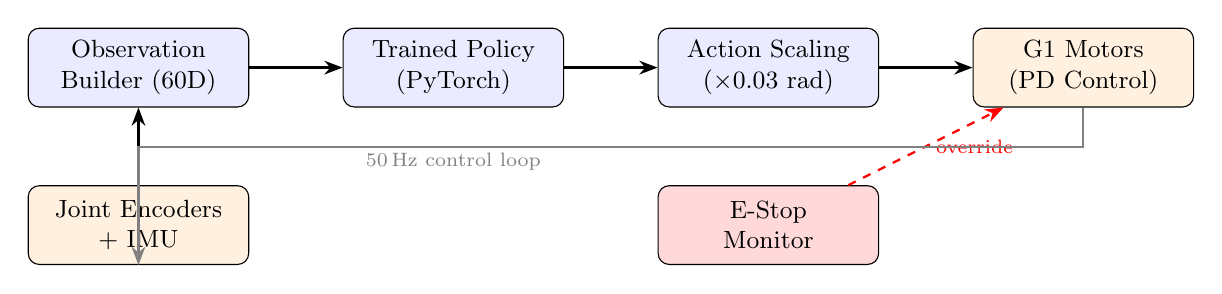
\begin{tikzpicture}[
  block/.style={draw, rounded corners, minimum width=2.8cm, minimum height=1cm, fill=blue!8, font=\small, align=center},
  hw/.style={draw, rounded corners, minimum width=2.8cm, minimum height=1cm, fill=orange!12, font=\small, align=center},
  arrow/.style={-Stealth, thick},
]
\node[block] (policy) at (0, 0) {Trained Policy\\(PyTorch)};
\node[block] (obs) at (-4, 0) {Observation\\Builder (60D)};
\node[block] (scale) at (4, 0) {Action Scaling\\($\times 0.03$ rad)};
\node[hw] (robot) at (8, 0) {G1 Motors\\(PD Control)};
\node[hw] (state) at (-4, -2) {Joint Encoders\\+ IMU};
\node[block, fill=red!15] (estop) at (4, -2) {E-Stop\\Monitor};

\draw[arrow] (obs) -- (policy);
\draw[arrow] (policy) -- (scale);
\draw[arrow] (scale) -- (robot);
\draw[arrow] (state) -- (obs);
\draw[arrow, dashed, red] (estop) -- (robot) node[midway, right, font=\scriptsize, text=red] {override};
\draw[arrow, gray] (robot.south) -- ++(0,-0.5) -| (state.south);

\node[font=\scriptsize, text=gray] at (0, -1.2) {50\,Hz control loop};
\end{tikzpicture}
\caption{Hardware deployment architecture. The policy runs inference on the robot's onboard computer (CPU), outputting joint position deltas at 50\,Hz. The E-stop monitor runs in a background thread, overriding motor commands if triggered.}
\label{fig:deployment}
\end{figure}

\subsection{Joint-Space Deployment}
The deployment script (\texttt{deploy\_g1\_joint\_space.py}) implements:
\begin{enumerate}[nosep]
  \item Load trained policy checkpoint (CPU inference).
  \item Initialize Unitree SDK2 communication via CycloneDDS.
  \item Build 60D observations from joint encoder readings and forward kinematics.
  \item Run policy inference at 50\,Hz (20\,ms cycle).
  \item Scale 14D action output by 0.03\,rad and clip to joint limits.
  \item Send joint position commands via low-level motor API.
\end{enumerate}

\noindent Hardware PD gains are set to approximately 50\% of simulation values (shoulders: $K_p=150$, $K_d=50$; wrists: $K_p=100$, $K_d=40$) to account for real-world compliance.

\subsection{Safety: Emergency Stop}
The E-stop system (\texttt{estop.py}) provides a critical safety mechanism:
\begin{itemize}[nosep]
  \item Background thread monitors spacebar key press.
  \item On trigger: reads current joint positions, sends high-damping commands ($K_d = 2\times$ normal, $K_p = 0$) to arrest motion.
  \item Maintains damping hold for 3 seconds, then exits.
  \item Integrated into the deployment control loop.
\end{itemize}

\subsection{Hardware Testing}

\begin{figure}[H]
\centering
% Placeholder for hardware photos
\fbox{\parbox{0.85\textwidth}{\centering\vspace{4cm}\textit{[FIGURE: Photos of G1 robot executing bimanual reaching on real hardware. Include: (a) robot reaching a left-side target, (b) robot reaching a right-side target, (c) both arms at different targets simultaneously.]}\vspace{4cm}}}
\caption{Hardware deployment of the trained joint-space policy on the Unitree G1 robot.}
\label{fig:hardware}
\end{figure}

%% ============================================================
\section{Discussion}
\label{sec:discussion}

\subsection{Key Lessons Learned}

\paragraph{1. Fixed penalties fight accuracy at all distances.}
Action-magnitude and wrist-position penalties create a constant cost that the policy must overcome, reducing the effective reward gradient for tracking. State-dependent rewards (proximity-scaled) are preferable, but must be compatible with the task requirements.

\paragraph{2. Action-based rewards are incompatible with orientation control.}
Any reward that penalizes action magnitude near the target---including \texttt{proximity\_action\_magnitude} and the action component of \texttt{terminal\_damping}---suppresses the wrist joint actions needed for orientation control. EE-velocity-based rewards are preferable for anti-jitter because they penalize the \emph{outcome} (unwanted movement) rather than the \emph{mechanism} (joint actions).

\paragraph{3. Shared networks create gradient imbalance in bimanual tasks.}
When two arms share a single actor network, whichever arm converges first generates disproportionately large gradients that dominate the shared weights, effectively starving the other arm. The bimanual balance reward ($\min$ aggregation) directly addresses this by ensuring the gradient always points toward improving the lagging arm.

\paragraph{4. tanh kernel saturation requires scale-appropriate $\sigma$.}
A tanh reward with $\sigma=0.5$\,rad has zero gradient at 1.7\,rad orientation error. Multi-level rewards with appropriately scaled $\sigma$ values are essential---analogous to multi-scale feature extraction in computer vision.

\paragraph{5. Position and orientation rewards must be balanced.}
With 27:1 position-to-orientation reward ratio, the policy rationally ignores orientation. The final 1.5:1 ratio (position per arm $\sim$32 vs.\ orientation per arm $\sim$27 + shared bimanual terms) achieves both sub-2$^\circ$ orientation and sub-6\,cm position accuracy.

\subsection{Limitations and Future Work}
\begin{itemize}[nosep]
  \item \textbf{Position accuracy}: The right arm at 5.8\,cm could be improved with longer training (the curve was still descending at 10K iterations) or a fine-tuning phase with higher position weights.
  \item \textbf{Jitter quantification}: Anti-jitter rewards are included but real-hardware jitter has not been systematically quantified.
  \item \textbf{Orientation range}: Target orientations are limited to $\pm$0.5\,rad ($\pm 29^\circ$). Larger ranges may require additional training or network capacity.
  \item \textbf{Dynamic targets}: Current targets are fixed per episode (resampled every 4--6\,s). Continuous trajectory tracking would require additional reward shaping.
  \item \textbf{Contact tasks}: This is a prerequisite for grasping and manipulation, which would require force/torque observations and contact-rich reward terms.
\end{itemize}

%% ============================================================
\section{Conclusion}
\label{sec:conclusion}

We developed a complete RL pipeline for bimanual 6-DOF reaching on the Unitree G1 humanoid, from initial IK-based prototypes through to direct joint-space policies deployed on real hardware. Through systematic iteration across 16+ training experiments, we identified and resolved critical issues in reward design, observation structure, workspace bounds, and bimanual learning dynamics.

The final policy achieves 1.7--5.8\,cm position error and 1.6--2.1$^\circ$ orientation error for both arms with randomized 6-DOF pose targets. The key innovations---bimanual balance rewards, multi-level orientation tracking, and the elimination of action-magnitude penalties for orientation-aware tasks---are broadly applicable to any shared-network bimanual RL system.

The trained policy runs at 50\,Hz on CPU hardware with a 330K-parameter MLP, demonstrating that sim-to-real transfer for bimanual reaching is practical with careful reward engineering and no runtime kinematic solver.

%% ============================================================
\section*{Code Availability}
The complete codebase is available in the \texttt{Amber-G1-Manipulation-RL} repository, structured as:
\begin{itemize}[nosep]
  \item \texttt{g1\_upper\_body\_tasks/g1\_tasks/reach\_g1\_upper\_body/} --- Environment configuration, rewards, and observations
  \item \texttt{g1\_upper\_body\_tasks/scripts/} --- Training, visualization, and deployment scripts
  \item \texttt{g1\_description/} --- Robot URDF/USD assets
  \item \texttt{checkpoints/} --- Trained model checkpoints
\end{itemize}

%% ============================================================
\begin{thebibliography}{9}
\bibitem{schulman2017ppo} J.~Schulman, F.~Wolski, P.~Dhariwal, A.~Radford, and O.~Klimov, ``Proximal Policy Optimization Algorithms,'' \textit{arXiv:1707.06347}, 2017.
\bibitem{isaaclab} NVIDIA, ``Isaac Lab: A Unified Framework for Robot Learning,'' 2024. Available: \url{https://isaac-sim.github.io/IsaacLab/}
\end{thebibliography}

\end{document}
